\chapter{Results}

\ifdraft{In this section you discuss any issues that came up while developing
the system.  If you found something particularly interesting,
difficult, or an important learning experience, put it here.  This is
also a good place to put additional figures and data.}

In this section we discuss the results of considering HLC within the game Breakthrough, using a Concept Activation vector for evaluating how the neural network recognizes the HLC's. We first take a look at the changes in ephasis of the neural network during training. The main point of interest there being whether the nerual network notices simple HLCs early then stops taking them into consideration as the network improves.

\section{Evaluating the improvements of the neural network over generations}

To test which HLC the neural network places its emphasis on during training we trained a neural network for $200$ iterations, taking snapshots of the network every $10$ generations. Then we had the neural network play against itself for $100$ games collecting the states it encountered during play. These states were then examined by a concept activation vector representing these HLCs. Firstly there is the numbers HLC, where the number of pawn the player has minus the number of pawns the opponent had, the breakpoint we selected was $2$ meaning that if you have $2$ more pawns then your opponent, you're in a position where a HLC called numbers advantage is present.

\begin{figure}[]
    \centering
    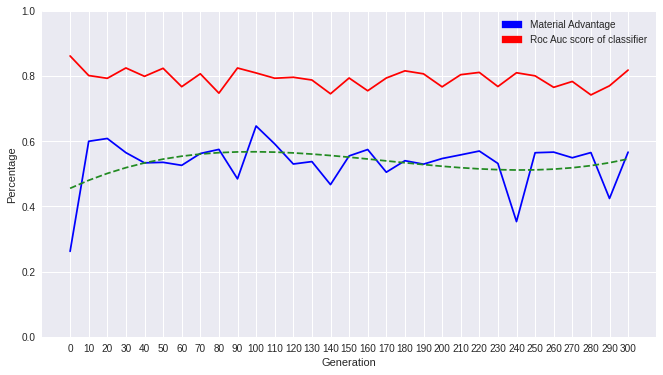
\includegraphics[width=0.7\textwidth]{graphics/number_pawns_trend}
    \caption{Percentage of selected states containing the HLC numbers advantage}
    \label{fig:numberadvantage}
\end{figure}

The Figure \ref{fig:numberadvantage}. shows that over the course of training the numbers advantage HLC is only ever a slight factor in the selection of states and we can say that the neural network doesn't really consider number advantage in its selection process.

The second HLC we examined was aggressiveness, that is a state in which you most advanced pawn is $2$ or more squares further than the opponents most advanced pawn. 

\begin{figure}[]
    \centering
    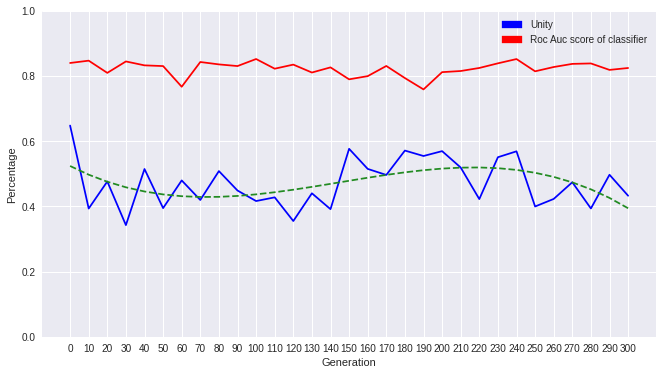
\includegraphics[width=0.7\textwidth]{graphics/most_advanced_trend.png}
    \caption{Percentage of selected states containing the HLC aggressiveness}
    \label{fig:aggressiveness}
\end{figure}

From Figure \ref{fig:aggressiveness}. we can see that the aggressiveness HLC is a growing factor over as the nerual network is trained. Generally when your opponent is not skilled this strategy is considered a good one.

The last HLC that we examined was unity, the unity HLC represents the absolute average distance of your pawns from the center row of your pawns. This HLC is calculated as the row of your furthest pawn from the starting row $r_{far}$, the row of your nearest pawn from the starting row $r_{near}$. Finding the middle row is then $\frac{r_{far} + r_{near}}{2}$, we then take the absolute of the average distance from the pawns to that row. To find the point at which this value relates to a state with the HLC unity, we sampled a myriad of states and decided on the value of $0.35$. The value of $0.35$ generally allows your states to have two rows that have the majority of the pawns and one or two pawns one row away from the group.

\begin{figure}[]
    \centering
    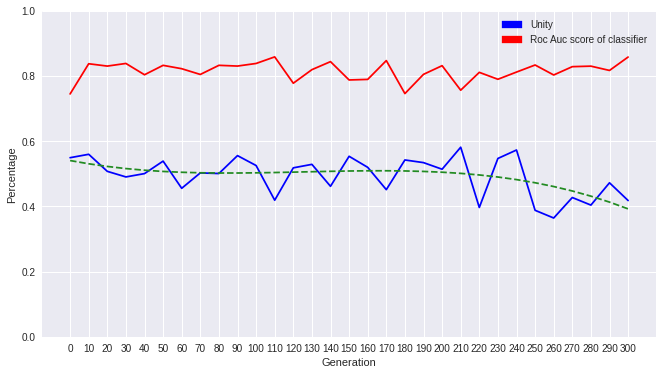
\includegraphics[width=0.7\textwidth]{graphics/unity_trend.png}
    \caption{Percentage of selected states containing the HLC aggressiveness}
    \label{fig:unity}
\end{figure}

The literature of breakthrough implies that being patient and waiting until your opponent makes a mistake is generally the preferred strategy for winning, and the concept activation vector for Unity is generally triggered, and increases with the amount of generations the neural network is trained for. These results imply that the neural network does infact recognize successful strategies, and focuses its training in the direction of the successful strategies.

